\usetikzlibrary{arrows, automata}

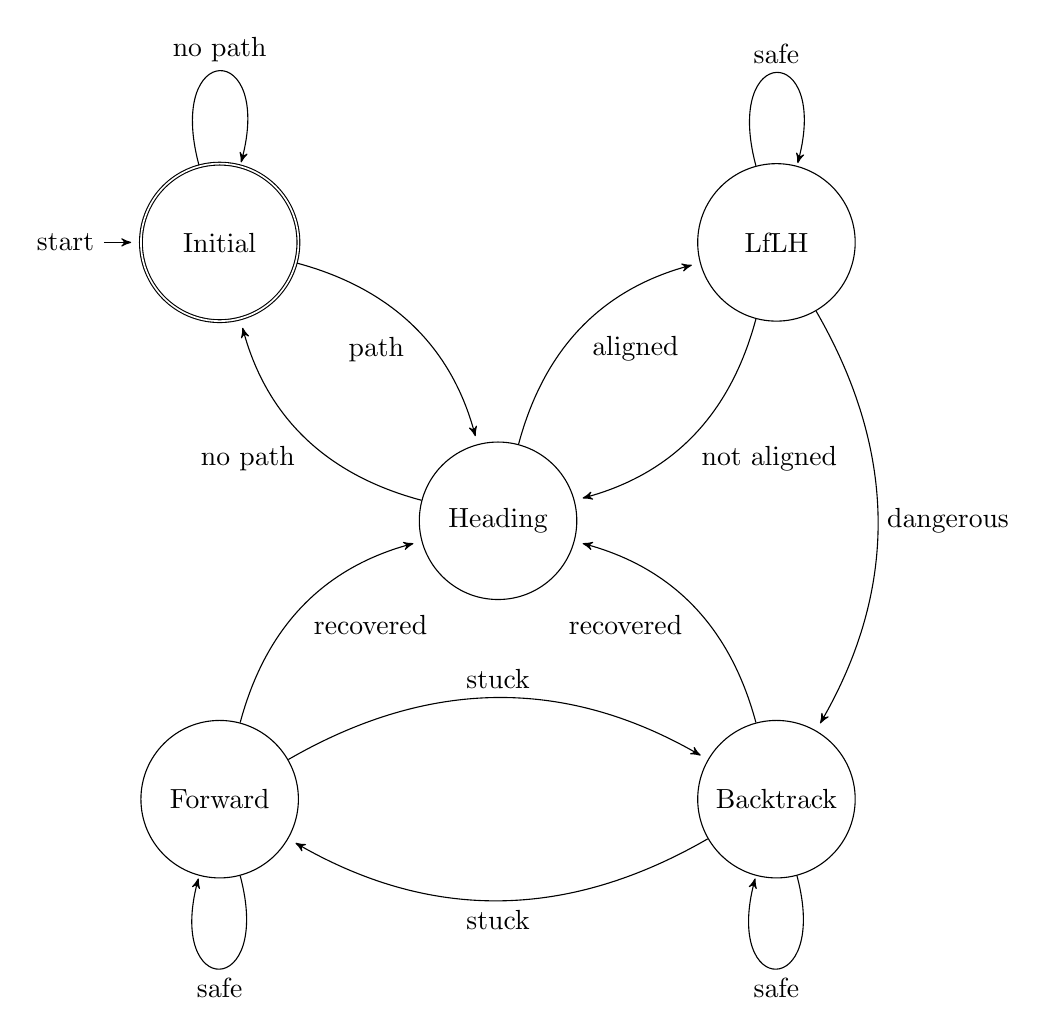
\begin{tikzpicture}[>=stealth', shorten >=3pt, auto, node distance=5cm]
     \node[initial,state, circle, accepting, minimum size=2.0cm]       (initial)     {Initial};
     \node[state, circle, minimum size=2.0cm]  (heading)   [below right of=initial]  {Heading};
     \node[state, circle, minimum size=2.0cm]  (LfLH)      [above right of=heading]  {LfLH};
     \node[state, circle, minimum size=2.0cm]  (backtrack) [below right of=heading]  {Backtrack};
     \node[state, circle, minimum size=2.0cm]  (forward)   [below left of=heading]   {Forward};

     \path[->] (initial)   edge [loop above]   node {no path}       (initial)
               (initial)   edge [bend left]    node[below left] {path}          (heading)
               % (heading)   edge [loop above]   node {not aligned}   (heading)
               (heading)   edge [bend left]    node {no path}       (initial)
               (heading)   edge [bend left]    node[below right] {aligned}       (LfLH)
               (LfLH)      edge [loop above]   node {safe}          (LfLH)
               (LfLH)      edge [bend left]    node {not aligned}   (heading)
               (LfLH)      edge [bend left]    node {dangerous}     (backtrack)
               (backtrack) edge [loop below]   node {safe}          (backtrack)
               (backtrack) edge [bend left]    node {stuck}         (forward)
               (backtrack) edge [bend right]   node {recovered}     (heading)
               (forward)   edge [loop below]   node {safe}          (forward)
               (forward)   edge [bend left]    node [below right] {recovered}     (heading)
               (forward)   edge [bend left]    node {stuck}         (backtrack);
\end{tikzpicture}